%%%%%%%%%%%%%%%%%%%%%%%%%%%%%%%%%%%%%%%%%
% Structured General Purpose Assignment
% LaTeX Template
%
% This template has been downloaded from:
% http://www.latextemplates.com
%
% Original author:
%  Ted Pavlic (http://www.tedpavlic.com)
% Modified by:
%  Joe Del Rocco (https://joe.delrocco.org)
%%%%%%%%%%%%%%%%%%%%%%%%%%%%%%%%%%%%%%%%%

%----------------------------------------------------------------------------------------
%  PACKAGES AND CONFIGURATION
%----------------------------------------------------------------------------------------

\documentclass[fleqn]{article}
\usepackage{xargs}
\usepackage{geometry}
\usepackage{fancyhdr} % For custom headers
\usepackage{lastpage} % To determine the last page for the footer
\usepackage{extramarks} % For headers and footers
\usepackage[most]{tcolorbox} % For problem answer sections
\usepackage{graphicx} % For inserting images
\usepackage{xcolor} % For link coloring
\usepackage[hidelinks]{hyperref} % For URL links (no box or color name)
\usepackage[permil]{overpic}
\usepackage{pict2e} % for drawing polygons
\usepackage{listings}

% Margins
\geometry{
a4paper,
tmargin=1in,
bmargin=1in,
lmargin=1in,
rmargin=1in,
textwidth=6.5in,
textheight=9.0in,
headsep=0.25in
}

% Header and footer
\pagestyle{fancy}
\lhead{\myName} % Top left header
\chead{\myAssignment} % Top center header
\rhead{\firstxmark} % Top right header
\lfoot{\lastxmark} % Bottom left footer
\cfoot{} % Bottom center footer
\rfoot{Page\ \thepage\ of\ \pageref{LastPage}} % Bottom right footer
\renewcommand\headrulewidth{0.4pt} % Size of the header rule
\renewcommand\footrulewidth{0.4pt} % Size of the footer rule

% Other configurations
\setlength\parindent{0pt} % Removes all indentation from paragraphs
\setlength\parskip{1pt} % Ensures paragraphs are still recognizable as such
\setcounter{secnumdepth}{0} % Removes default section numbers
\setcounter{tocdepth}{3} % Sets depth of table of contents
\linespread{1.1}

% Code highlight
\definecolor{light-gray}{gray}{0.9}
\newcommand{\code}[1] {\colorbox{light-gray}{\texttt{#1}}}

% Template values
\newcommand{\myLogo}{img/starfleet.jpg}
\newcommand{\myName}{Jean-Luc Picard}
\newcommand{\myJobTitle}{Cadet, First Class}
\newcommand{\myCompany}{Starfleet Academy}
\newcommand{\myLocation}{1701 Lincoln Blvd, San Francisco}
\newcommand{\myURL}{www.starfleet.edu}
\newcommand{\myEmail}{jpicard@student.starfleet.edu}
\newcommand{\myCourse}{COT\ 6410}
\newcommand{\mySection}{Spring 2325}
\newcommand{\myTeacher}{Dr. Vassbinder}
\newcommand{\myAssignment}{Using \LaTeX{} Package \code{overpic}}
\newcommand{\myDueDate}{Thursday,\ February\ 26,\ 2325}

%----------------------------------------------------------------------------------------
%  DOCUMENT STRUCTURE (MACROS & ENVIRONMENTS)
%----------------------------------------------------------------------------------------

% Colored links macro
\newcommand{\hrefcol}[3] {\href{#1}{\textcolor{#3}{#2}}}

% Creates a counter to keep track of the number of problems
\newcounter{homeworkProblemCounter}

% Macro for custom title page signature header
\newsavebox{\myTitleSignature}
\sbox{\myTitleSignature}{%
\begin{tabular*}{\textwidth}{@{}l@{}|@{\extracolsep{0.125in}}l@{}}%
\parbox{4.25in}{\raggedright{\includegraphics{\myLogo}}} &
\parbox[c][]{2.25in}{{\textbf{\myName} \par}
                    {\small \myJobTitle \par}
                    {\small \myCompany \par}
                    {\small \myLocation \par}
                    {\small \hrefcol{https://\myURL}{\myURL}{blue} \par}
                    {\small \hrefcol{mailto:\myEmail}{\myEmail}{blue}} \par}
\end{tabular*}}

% Header and footer for when a page split occurs within a problem environment
\newcommand{\enterProblemHeader}[1]{%
\nobreak%\extramarks{#1}{#1 continued on next page\ldots}\nobreak%
\nobreak%\extramarks{#1 (continued)}{#1 continued on next page\ldots}\nobreak%
}

% Header and footer for when a page split occurs between problem environments
\newcommand{\exitProblemHeader}[1]{%
\nobreak%\extramarks{#1 (continued)}{#1 continued on next page\ldots}\nobreak%
\nobreak%\extramarks{#1}{}\nobreak%
}

\newcommand{\homeworkProblemName}{} % Argument = name of problem; default = "Problem #"
\newenvironment{homeworkProblem}[1][Problem \arabic{homeworkProblemCounter}]{%
\stepcounter{homeworkProblemCounter}% % Increase counter for number of problems
\renewcommand{\homeworkProblemName}{#1}% % Assign \homeworkProblemName the argument
\section{\homeworkProblemName}% % Make a section in the document with the custom problem count
\enterProblemHeader{\homeworkProblemName}% % Header and footer within environment
}{%
\exitProblemHeader{\homeworkProblemName}% % Header and footer after environment
}

\newcommandx{\problemAnswer}[2][1=Answer]{%
%\newcommand{\problemAnswer}[2][#1,Answer]{% % Defines the problem answer command
\begin{tcolorbox}[breakable,enhanced,colback=gray!5!white,title=#1]%
#2
\end{tcolorbox}%
% Alternative - Makes the box around the problem answer and puts the content inside
%\noindent\framebox[\columnwidth][c]{\begin{minipage}{0.98\columnwidth}#1\end{minipage}}
}

\newcommand{\homeworkSectionName}{}
\newenvironment{homeworkSection}[1]{% % For sections w/in problems; Argument = name of section (no default)
\renewcommand{\homeworkSectionName}{#1}% % Assign \homeworkSectionName the argument
\subsection{\homeworkSectionName}% % Make a subsection with the name of the subsection
\enterProblemHeader{\homeworkProblemName\ [\homeworkSectionName]}% % Header and footer within environment
}{%
\enterProblemHeader{\homeworkProblemName}% % Header and footer after environment
}

%----------------------------------------------------------------------------------------
%  TITLE PAGE
%----------------------------------------------------------------------------------------
\begin{document}

% Blank out the traditional title page
\title{\vspace{-1in}} % no title name
\author{} % no author name
\date{} % no date listed
\maketitle % makes this a title page

% Use custom title macro instead
\usebox{\myTitleSignature}
\vspace{1in} % spacing below title header

% Assignment title
{\centering \huge \myAssignment \par}
{\centering \noindent\rule{4in}{0.1pt} \par}
\vspace{0.05in}
{\centering \myDueDate \par}
\vspace{1in}

% Table of Contents
\tableofcontents
\vspace{0.5in}

\begin{homeworkProblem}[Where's the code?]
Instead of textualizing the \LaTeX~in this document, as was done originally (and which was difficult to copy and paste), it is recommended that you just inspect the code directly. If you found this template on \hrefcol{https://www.overleaf.com}{Overleaf}{blue}, you can see the code already in the editor. If you happened upon this example as a document, the  \hrefcol{https://github.com/delrocco/overpic-example}{code is in this repository}{blue}. Please feel free to steal anything that helps you :).
\vspace{0.1in}
%\problemAnswer[Code]{Just view the \LaTeX~code in the repository.}
\end{homeworkProblem}

\newpage

%----------------------------------------------------------------------------------------

\begin{homeworkProblem}[How do I overlay text onto an image?]

\problemAnswer[Result]{
\frame{
\begin{overpic}[width=0.5\textwidth]{img/salmon.jpg}%
\put(20,600) {Salmon sashimi with sesame seeds and lemon}%
\put(750,350){lemon}%
\put(300,500){seeds}%
\put(200,150){salmon}%
\put(550,50){Looks yummy, right?}%
\end{overpic}
}
}

\end{homeworkProblem}

%----------------------------------------------------------------------------------------

\begin{homeworkProblem}[How do I superimpose a grid for easy alignment?]

\problemAnswer[Result]{
\vspace{0.1in}
\hspace{0.1in}
\begin{overpic}[width=0.5\textwidth,grid]{img/salmon.jpg}%
\put(750,350){lemon}%
\end{overpic}
}

\end{homeworkProblem}

%----------------------------------------------------------------------------------------

\begin{homeworkProblem}[How do I draw cirles, lines and polygons over an image?]

\problemAnswer[Result]{
\frame{
\begin{overpic}[width=0.5\textwidth]{img/salmon.jpg}%
\put(800,380){\color{blue}lemon}%
\put(700,300){\color{blue}\circle{200}}%
\put(100,600){seeds}%
\put(150,585){\linethickness{0.25mm}\color{black}\line(1,-1){285}}%
\put(10,230){salmon}%
\multiput(180,240)(50,0){4}{\linethickness{0.5mm}\line(1,0){30}}%
\put(450,600){kaiware daikon sprouts}%
\put(450,450){\linethickness{0.25mm}\color{black}\polygon(0,0)(290,0)(290,120)(0,120)}%
\put(280,55){\circle*{10}}%
\put(280,55){\circle{20}}%
\put(300,40){Looks yummy, right?}%
\end{overpic}
}
}

\end{homeworkProblem}

%----------------------------------------------------------------------------------------

\begin{homeworkProblem}[How do I superimpose images over an image?]

\problemAnswer[Result]{
\begin{overpic}[width=0.5\textwidth]{img/salmon.jpg}%
\put(500,300){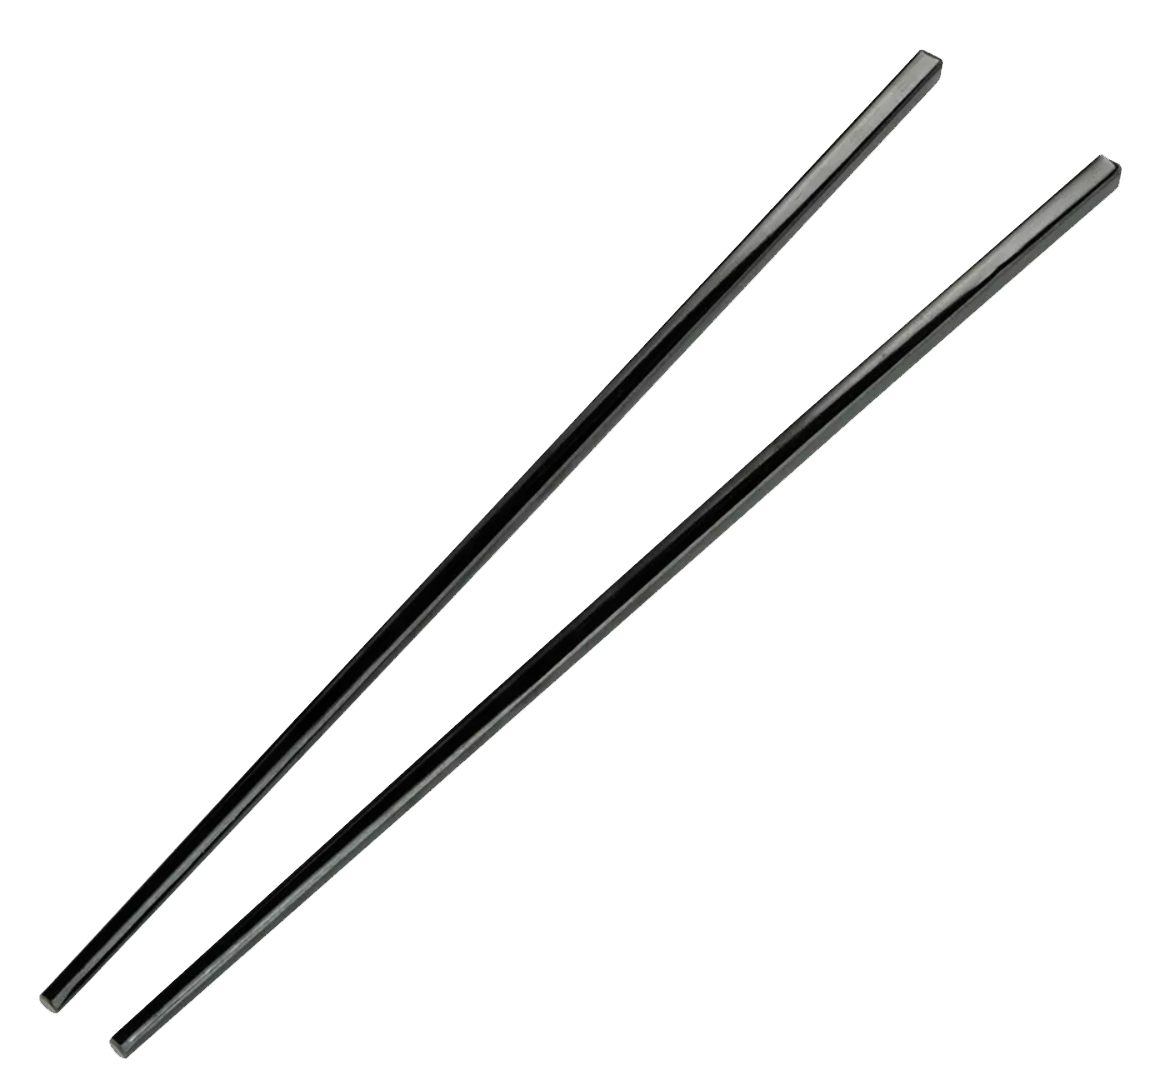
\includegraphics[width=0.3\textwidth]{img/chopsticks.png}}%
\end{overpic}
%\vspace{0.25in}
}

\end{homeworkProblem}

%----------------------------------------------------------------------------------------

\begin{homeworkProblem}[How do I use this to compare multiple images in a figure?]

\problemAnswer[Result]{

\frame{\begin{overpic}[width=0.3\textwidth]{img/salmon.jpg}%
\put(20,590){(A)}%
\end{overpic}}%
~%
\frame{\begin{overpic}[width=0.3\textwidth]{img/salmon.jpg}%
\put(20,590){(B)}%
\end{overpic}}%

}

\problemAnswer[Result]{

\frame{\begin{overpic}[width=0.215\textwidth]{img/salmon.jpg}%
\put(20,550){(a)}%
\end{overpic}}%
~%
\frame{\begin{overpic}[width=0.215\textwidth]{img/salmon.jpg}%
\put(20,550){(b)}%
\end{overpic}}%
~%
\frame{\begin{overpic}[width=0.215\textwidth]{img/salmon.jpg}%
\put(20,550){(c)}%
\end{overpic}}%
~%
\frame{\begin{overpic}[width=0.215\textwidth]{img/salmon.jpg}%
\put(20,550){(d)}%
\end{overpic}}%

}

\problemAnswer[Result]{

\frame{\begin{overpic}[width=0.6\textwidth]{img/salmon.jpg}%
\put(650,10){\frame{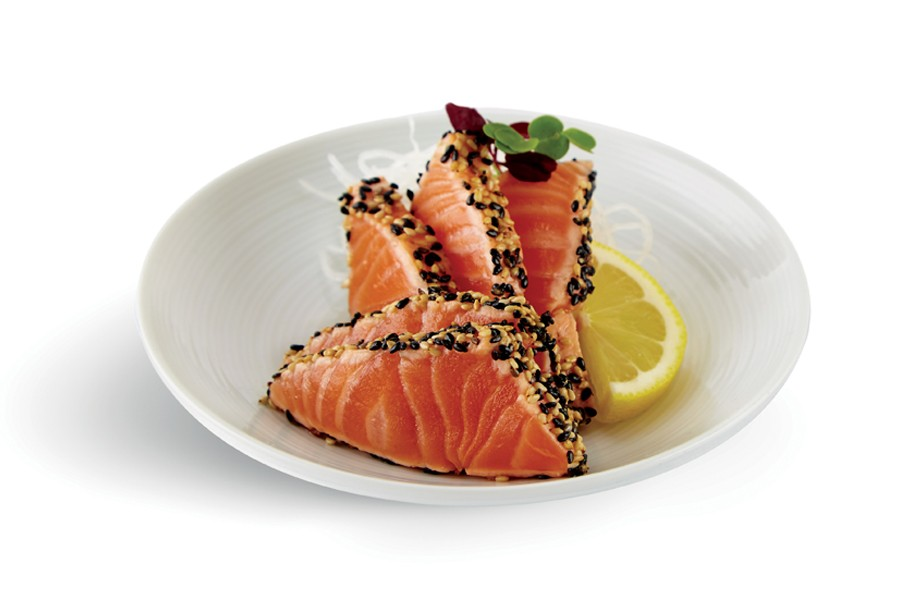
\includegraphics[width=0.2\textwidth]{img/salmon.jpg}}}%
\put(10,620){(1)}%
\put(660,190){(2)}%
\end{overpic}}%

}

\end{homeworkProblem}

%----------------------------------------------------------------------------------------

\newpage
\begin{homeworkProblem}[What else can I do with overpic?]
\problemAnswer{
Here is another 1-page primer by Rolf Niepraschk to get you started:\\
\hrefcol{http://www.ctex.org/documents/packages/graphics/opic-rel.pdf}{http://www.ctex.org/documents/packages/graphics/opic-rel.pdf}{blue}\\
\\
Here is the official documentation on CTAN:\\
\hrefcol{http://mirrors.ibiblio.org/CTAN/macros/latex/contrib/overpic/overpic.pdf}{http://mirrors.ibiblio.org/CTAN/macros/latex/contrib/overpic/overpic.pdf}{blue}\\
\\
Here is a relevant thread on the TeX StackExchange:\\
\hrefcol{https://tex.stackexchange.com/questions/20792/how-to-superimpose-latex-on-a-picture}{https://tex.stackexchange.com/questions/20792/how-to-superimpose-latex-on-a-picture}{blue}\\
\\
You can also use TikZ, but it is more complicated:\\
\hrefcol{https://tex.stackexchange.com/questions/9559/drawing-on-an-image-with-tikz}{https://tex.stackexchange.com/questions/9559/drawing-on-an-image-with-tikz}{blue}\\
}

\end{homeworkProblem}

\end{document}
